Die \textit{Foundation for Intelligent Physical Agents} (FIPA) der \textit{IEEE Computer Society} hat im Bereich des Multi-Agenten-Systems mehrere Standards erarbeitet. Diese Standards beschreiben alle grundlegenden Elemente und Funktionen, die für eine Multi-Agenten-Plattform benötigt werden. \cite{article:flexibleSoftware}

Es gibt einige Projekte, die diesen Standard implementieren \cite{web:fipaList}. Unter diesen eignet sich das \textit{Java Agent Development Framework} (JADE) am besten für dieses Projekt. Zum einen ist das JADE Framwork in \textit{Java} implementiert und somit plattformunabhängig \cite{web:java}. Es ist open-source. Es kann also eigenständig verändert und erweitert werden. Zudem ist die Benutzung des Frameworks nicht mit Lizenzkosten verbunden. Zuletzt ist JADE in Form von \cite{book:jade} detailliert beschrieben.

In den folgenden Kapiteln wird eine Auswahl wichtiger Grundkonzepte des JADE Framworks vorgestellt. 

\subsection{Grundlagen}
\label{chap:jade_grundlagen}
\begin{figure}[H]
    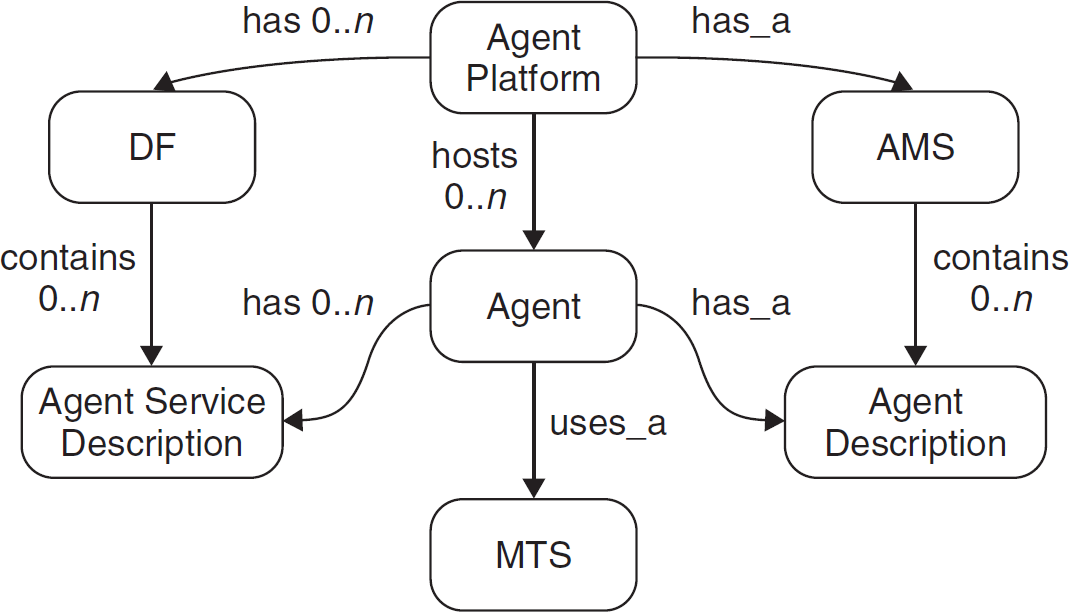
\includegraphics[width=10cm]{images/jade_structure.png}
    \centering
    \caption{\textit{Entity-Relationship}-Diagramm aus \cite{book:jade}}
    \label{fig:jade_structure}
\end{figure}

\paragraph{\textit{Agent Platform} (AP)}
Die AP beschreibt die physikalische Infrastruktur in der die Agenten ausgeführt werden. Hier sind die Rechner, die Netzwerke, die Betriebssysteme, das \textit{Agent Management System}, die Agenten selbst und zusätzliche Software mit inbegriffen.

\paragraph{Agent}
Ein Agent existiert in der AP und bietet ein oder mehrere Services die mit Hilfe einer \textit{Service Description} veröffentlicht sind. Ein Agent hat ein eindeutigen \textit{FIPA Agent Identifier} (AID).  

\paragraph{Diretory Faciliator (DF)}
Der DF ist eine optionale Komponente. Der DF stellt den Agenten einen "'Gelbe Seiten"'-Service zur Verfügung und hält eine komplette Liste aller Agenten. Der "'Gelbe Seiten"'-Service wird von den Agenten genutzt um ihre Services zu registrieren und somit den anderen Agenten verfügbar zu machen. Die AP kann beliebig viele DF starten, die ihre Daten untereinander synchronisieren.

\paragraph{Agent Management System (AMS)}
Das AMS ist für das Erstellen und Löschen der Agenten verantwortlich. Jeder Agent muss sich beim AMS registrieren. Bei diesem Schritt vergibt das AMS dann die AID für die Agenten. Ein Agent beendet sich, wenn er sich vom AMS abmeldet. Das AMS ist als eine Entität zu verstehen und erstreckt sich auch über mehrere Rechner.

\paragraph{Message Transport Service (MTS)} Dieser Service wird von der AP bereitgestellt. Über ihn können die Agenten Nachrichten austauschen.
%
\subsection{Behaviour}
\label{chap:jade_agent}
Ein \textit{Behaviour} ist eine Aufgabe die ein Agent ausführen kann und als erbende Klasse von \texttt{jade.core.behaviours.Behaviour} implementiert ist. Für jeden Agenten startet die JADE Umgebung einen Thread. Ein \textit{Behaviour} wird über einen Scheduler auf diesem Thread ausgeführt. Der Agent fügt ein \textit{Behaviour} mit \texttt{addBehaviour()} der Scheduling-Queue hinzu. Dies kann der Agent während der Initialisierungsphase in der \texttt{steup()} Methode tun oder innerhalb eines \textit{Behaviours}. Jede \textit{Behaviour}-Subklasse muss die \texttt{action()} und \texttt{done()} Methode implementieren. Die \texttt{action()} Methode enthält die Logik, also den auszuführenden Code, des \textit{Behaviours}. Die \texttt{done()} Methode gibt einen \texttt{boolean} zurück, der Aussage darüber trifft, ob das \textit{Behaviour} seine Aufgabe abgeschlossen hat und damit aus Scheduling-Queue entfernt werden soll. Ein Agent kann mehrere \textit{Behavoiur} ausführen. Ein \textit{Behavoiur} ist jedoch nicht preemptive. Wenn die \texttt{action()} Methode vom Scheduler aufgerufen wird, kann diese nicht unterbrochen werden. Das \textit{Behaviour} muss also selbständig diese Ressource wieder freigeben. \cite{book:jade}

Das JADE Framwork stellt jedoch nicht nur den Basistypen zur Verfügung, sondern implementiert weitere abstrakte \textit{Behaviour}. Folgend wird eine Auswahl aus \cite{book:jade} vorgestellt.

\paragraph{One-Shot Behaviour}
Für das \texttt{jade.core.behaviours.OneShotBehaviour} muss eine erbende Klasse nur die \texttt{action()} Methode implementieren. \texttt{done()} liefert standardmäßig \texttt{true} zurück. Ein \textit{One-Shot Berhaviour} wird also nur einmal ausgeführt.

\paragraph{Cyclic Behaviour}
Das \texttt{jade.core.behaviours.CyclicBehaviour} ist dem \textit{One-Shot Behaviour} recht ähnlich. Die \texttt{done()} Methode liefert jedoch standardmäßig \texttt{false} zurück. Ein \textit{Cyclic Behaviour} beendet sich also nie.

\paragraph{Ticker Behaviour}
Das \texttt{jade.core.behaviours.TickerBehaviour} implementiert sowohl \texttt{action()} als auch \texttt{done()} Methoden. Die \texttt{done()} Methode liefert immer \texttt{false} zurück. Die \texttt{action()} Methode führt die \texttt{onTick()} Methode periodisch aus. Das Zeitintervall wird über den Konstruktor definiert. Das \textit{Ticker Behavior} ist selbst eine abstrakte Klasse. Erbende Klassen implementieren die Methode \texttt{onTick()}.
%
\subsection{Kommunikation}
\label{chap:jade_kommunikation}
Agenten interagieren miteinander. Dies geschieht indirekt über das Verändern der Umwelt oder durch direkte Kommunikation. Die direkte Kommunikation ist wahrscheinlich eines des wichtigsten Funktionen des JADE Frameworks. Die Kommunikation zwischen Agenten erfolgt durch den asynchronen Nachrichtenaustausch. Jeder Agent besitzt eine Queue in der alle Nachrichten eines Agenten empfangen werden. Eine Nachricht hält dabei mehrere Felder:
\begin{itemize}
\item Die ID des \textbf{Senders}
\item Eine Liste, die alle \textbf{Empfänger} enthält.
\item Die \textbf{Absicht} der Nachricht. Die FIPA definiert hier eine Liste mit Möglichkeiten. Zum Beispiel "'Inform"'. Der Sender berichtet den Empfänger einen Fakt.
\item Den \textbf{Inhalt}, den der Sender mitteilen möchte.
\item Die \textbf{Kodierung} der Nachricht. So das die Empfänger wissen, wie die Nachricht zu lesen ist.
\end{itemize} \cite{book:jade}
